\section{Faltung (Convolution)} 
\label{sec:convolution}
In \ref{sec:signals_and_systems} haben wir für Lineare Zeit-invariante Systeme definiert, dass sie sich vollständig durch ihre Impulsantwort
charakterisieren lassen. In diesem Abschnitt werden auf diese Tatsache genauer eingehen, und dabei definieren, was die Impulsantwort eigentlich
ist. Wir werden außerdem zeigen, wie die Impulsantwort eines Systems auf ein Signal angewendet wird, um den Effekt des Systems auf das Signal
zu erzeugen.

Eine beliebige Reihe (also ein beliebiges diskretes Signal) kann laut \ref{sec:signals_and_systems}
als Summe von skalierten und verzögerten Einheitsimpulsen dargestellt werden kann.
Oppenheim formuliert zur Präzisierung eine allgemeine Summenformel, mit der eine beliebige Reihe $x[n]$ ausgedrückt werden:
\begin{equation}
    x[n]=\sum_{k=-\infty}^\infty x[k]\delta[n-k]
    \label{eq:scaled_unit_sum}
\end{equation}
Die mathematische Beschreibung der diskreten Faltung leitet Oppenheim daraus wie folgt ab: 

Sei $y[n]$ das Ausgangssignal eines LTI-Systems, resultierend aus einem Eingangssignal $x[n]$. Sei $h_k[n]$ die Antwort eines Systems
auf einen Einheitsimpuls an Index $n=k$. Es gilt:

\begin{equation}
    y[n]=T\left( \sum_{k=-\infty}^{\infty}x[k]\delta[n-k] \right).
\end{equation}

Nach Superposition (Linearität) gilt auch:

\begin{equation}
    y[n]=\sum_{k=-\infty}^{\infty}x[k]T(\delta[n-k])=\sum_{k=-\infty}^{\infty}x[k]h_k[n].
    \label{eq:timevariant_equation}
\end{equation}
In Gleichung \ref{eq:timevariant_equation} ist $h_k[n]$ vom Laufindex der Summenfunktion abhängig. Es würden für die Berechnung der Summe also
genauso viele System-Antworten benötigt, wie Summierungen ausgeführt werden.
Unter Forderung der Zeitinvarianz des Systems fällt diese Eigenschaft weg:

\begin{equation}
    y[n]=\sum_{k=-\infty}^{\infty}x[k]h[n-k].
    \label{eq:convolution_sum}
\end{equation}
Die Gleichung \ref{eq:convolution_sum} wird als \textit{Faltungssumme} (engl.: \textit{Convolution Sum}) bezeichnet \cite[Seite 22f]{oppenheim1999}. Als kürzere Schreibweise für 
die Faltung zweier Signale $x$ und $h$ zu einem Ausgangssignal $y$ verwenden wir die Schreibweise $y[n]=x[n]*h[n]$.

Um das Prinzip der Faltung zu veraunschaulichen, werden wir nun einen der simpleren Anwendungsfälle betrachten: einen Tiefpassfilter.
Visualisierungen in diesem Abschnitt sind an die Grafiken von Richard Lyons \cite{lyons2010} angelehnt.
Dieser kann in der diskreten Zeitdomäne durch ein von Lyons \cite{lyons2010} \textit{Moving Averager} genannte System realisiert werden. Die Idee ist,
für jedes $n$-te Sample des Ausgangssignals einen Mittelwert aus mehreren Samples in der Umgebung des Index $n$ des Eingangssignals zu verwenden. Da die für jedes Ausgangs-Sample
eine um dieses Sample herum angeordnete Gruppe an Samples gemittelt wird, "bewegt" sich das Fenster der in die Mittelwertberechung einbezogenene Samples mit dem berechneten
Ausgangs-Sample, was den Namen Moving Averager begründet. Ein anderer Name für diese Art von Filter ist \textit{Transversalfilter} \cite{lyons2010}.
Tiefpassfilter dämpfen die höheren Frequenzen des Spektrums eines Signals. Das Wirkungsprinzip bei einem Moving Average Tiefpassfilters
beruht darauf, dass bei der Berechnung von Durchschnittswerten die schnellen Veränderungen der enthaltenen höheren Frequenzen durch die Mittelwertberechnung stärker beeinflusst
werden, als die langsamen Veränderungen der niedrigfrequenten Anteile des Spektrums. 
Da in der Signalverarbeitung oft Echtzeitberechnungen nötig sind, kann die intuitiv sinnvoll erscheinende Wahl von einer bestimmten Anzahl Samples vor und nach dem Index des zu berechnenden Ausgangs-Samples
nicht zuverlässig berechnet werden, denn ggf. existieren die Samples mit höherem Index noch nicht. Daher werden Samples mit kleinerem Index, also ältere Samples, für die 
Durchschnittswertberechnung genutzt. Bei einer Berechnung des Mittelwerts von 5 Samples gilt also 
\begin{equation}
    y[n]=\frac{1}{5}\sum_{k=0}^4x[n-k]\iff y[n]=\sum_{k=0}^4\frac{1}{5}x[n-k].
    \label{eq:mov_avg_filter}
    \cite{lyons2010}
\end{equation}
Die Summenformel zur Berechnung der Ausgangs-Samples unseres Moving Average Filters \ref{eq:mov_avg_filter} weist starke Ähnlichkeit mit der der Faltungssumme \ref{eq:convolution_sum} auf.
Die beiden auffälligsten Unterschiede sind die endliche Summierung und die Verwendung eines festen Koeffizienten, anstelle verschiedener Samples eines zweiten Signals.
In der Definition eines diskreten Signals ist aber nirgends festgelegt, dass verschiedene Samples unterschiedliche Werte haben müssen. Wir können folglich den für jeden Summanden
verwendeten Faktor $\frac{1}{5}$ auch als ein diskretes Signal, bestehend aus 5 Samples, mit den Werten $\frac{1}{5}$ interpretieren:
\begin{equation}
    \label{eq:fir_convsum}
    y[n]=\sum_{k=0}^4h[k]x[n-k]\text{ mit }h=\left(\frac{1}{5},\,\frac{1}{5},\,\frac{1}{5},\,\frac{1}{5},\,\frac{1}{5}\right).
\end{equation}
Die Summenformel \ref{eq:fir_convsum} ist eine endliche Faltungssumme. Es fällt auf, dass die Indizierung von Eingangs-Signal und Impulsantwort vertauscht sind, aufgrund der 
Kommutativen Eigenschaft der Faltung \cite{oppenheim1999} ist \ref{eq:fir_convsum} Äquivalent zu \ref{eq:convolution_sum}. Man nennt solche Filter \textit{Finite Impulse Response Filter},
kurz \text{FIR-Filter}. Die Filterkoeffizienten der Mittelwertberechnung sind dabei, wie schon durch die Notation als $h$ impliziert, die Impulsantwort des Systems, das unser
Moving Averager bildet. Um das Ergebnis des Moving Averagers zu veranschaulichen, betrachten wir ein Signal aus 3 zusammengesetzten Sinusschwingungen:

\begin{figure}[htbp]
    \centering
    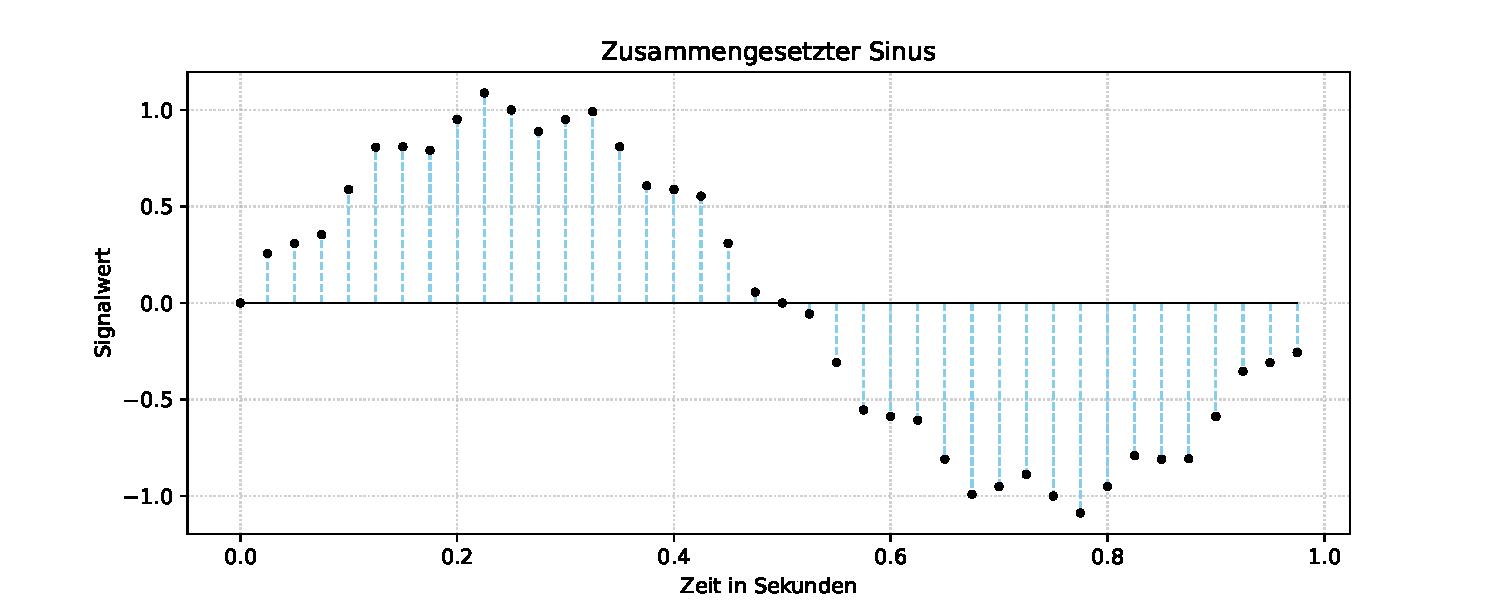
\includegraphics[width=0.5\textwidth]{graphic/python/chapter3/compound_sinusoid.pdf}
    \caption{Ein diskretes Signal, zusammengesetzt aus Sinusschwingungen mit den Frequenzen $f_0=1\,\text{Hz}$, $f_1=10\,\text{Hz}$, und $f_2=20\,\text{Hz}$}
    \label{fig:comp_sinusoid}
\end{figure}

Die Anwendung des Moving Averagers resultiert in einer deutlich sichtbaren Glättung des Signals, aber auch zu einer Verzögerung des Signals:

\begin{figure}[htbp]
    \centering
    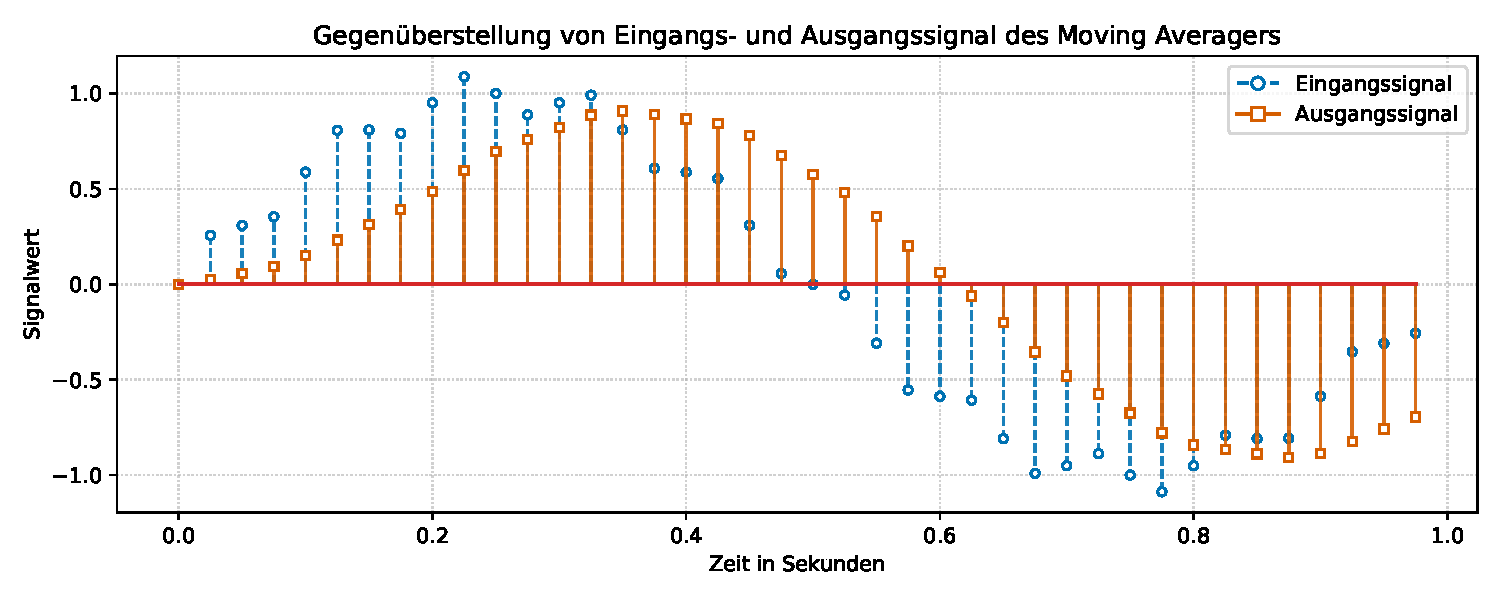
\includegraphics[width=0.5\textwidth]{graphic/python/chapter3/comparison_compound_filtered.pdf}
    \caption{}
    \label{fig:in_out_comparison}
\end{figure}

Der hier betrachtete FIR-Filter ist ein gutes Beispiel zur Veranschaulichung des Faltungsprozesses und seiner möglichen Auswirkungen. 
Die Faltungssumme selbst ist aber in allen anderen Anwendungsbereichen von Faltungsprozessen in der Signalverarbeitung gleich. In echten 
Anwendungsfällen werden jedoch in der Regel Impulsantworten und Signale mit weit höheren Längen, also auch weit mehr Summanden und Multiplikationen
pro berechnetem Ausgangs-Sample, verwendet. Dies bringt seine eigenen Herausforderungen mit sich, denn besonders in Echtzeitanwendungen ist
eine hinreichend schnelle Berechnung der Ausgangssamples nicht verhandelbar. Bei der häufig auftretenden Abtastrate von 44,1kHz bleiben für
die Berechnung eines Blockes von 256 Ausgangs-Samples weniger als 6 Millisekunden. Daher stellen wir abschließend ohne Beweis eine in der
praktischen Anwendung außerordentlich wichtige Eigenschaft der Faltung vor.


\subsection{Das Convolution-Theorem}
\label{sec:convolution_theorem}
Seien $X(e^{i\omega})$, $H(e^{i\omega})$ und $Y(e^{i\omega})$ die diskreten Fourier-Transformationen des Eingangssignals $x$, der Impulsantwort $h$, und 
des Ausgangssignals $y$ einer Faltung $y[n]=x[n]*h[n]$. Dann gilt:

\begin{equation}
    \label{eq:convolution_theorem}
    Y(e^i\omega)=X(e^i\omega)\cdot H(e^i\omega).
\end{equation} 
Die Faltung zweier Signale in der Zeitdomäne ist äquivalent zu einer Multiplikation der Signale in der Frequenzdomäne. Mit einer inversen diskreten Fourier-Transformation
des Ausgangs-Spektrums $Y(e^i\omega)$ erhalten wir das Ausgangssignal in der Zeitdomäne \cite{oppenheim1999}. Das heißt, bei hinreichend effizienter Berechnung der (inversen) diskreten Fourier-Transformationen
können wir auf die aufwändige direkte Berechnung der Faltungssume verzichten und stattdessen dasselbe Ergebnis durch Multiplikation in der Frequenzdomäne erzielen!